\documentclass[12pt, a4paper]{article}
\usepackage[margin=1in]{geometry}
\usepackage{graphicx}
\usepackage{natbib}
\usepackage[utf8]{inputenc}
\usepackage{amsmath}
\usepackage{amssymb}
\usepackage{float}

\title{The Awakened Population in South Korea: Demographics, Abilities, and Social Integration}
\author{Seunghoon Kim\footnote{Department of Supernatural Studies, Seoul National University, Seoul, South Korea} \and Jiyoung Lee\footnote{Institute for Social Integration Research, Korea University, Seoul, South Korea}}
\date{May 2027}

\begin{document}

\maketitle

\begin{abstract}
This study presents a comprehensive analysis of the awakened population in South Korea, focusing on their demographic characteristics, the nature and distribution of their abilities, and the challenges they face in social integration. Drawing upon a nationwide survey and in-depth interviews with awakened individuals, the authors provide insights into the age, gender, and socioeconomic profiles of this unique population segment. The findings reveal a wide range of abilities among the awakened, from enhanced physical capabilities to psychokinetic powers, with a small subset of individuals possessing abilities of extraordinary strength and complexity. The paper also examines the social and cultural barriers encountered by the awakened, including stigma, discrimination, and the pressure to conform to societal expectations. The authors discuss the implications of these findings for policymakers and social support services, highlighting the need for inclusive and responsive measures to foster the well-being and integration of the awakened population in South Korea.
\end{abstract}

\section{Introduction}
The 2025 catastrophe, which saw the sudden emergence of portals leading to treacherous dungeons filled with powerful creatures, has had a profound impact on societies worldwide \citep{nakamura2027rise}. In the aftermath of this event, a small portion of the population has awakened with extraordinary abilities, ranging from enhanced physical capabilities to psychokinetic powers \citep{lee2027psychological}. These individuals, known as the awakened, have become key actors in the exploration of dungeons and the defense against the creatures that emerge from them \citep{kim2027emergence}.

In South Korea, the awakened population has been at the forefront of the country's response to the post-catastrophe reality. Hunter guilds, composed primarily of awakened individuals, have taken on the responsibility of exploring the dungeons that have appeared across the country and combating the threats that emanate from them \citep{seo2027shamanism}. However, despite their crucial role in protecting society, the awakened population faces significant challenges in terms of social integration and acceptance \citep{lee2027psychological}.

This study aims to provide a comprehensive analysis of the awakened population in South Korea, focusing on their demographic characteristics, the nature and distribution of their abilities, and the barriers they face in social integration. By drawing upon a nationwide survey and in-depth interviews with awakened individuals, the authors seek to contribute to a better understanding of this unique population segment and inform policies and support services that can foster their well-being and inclusion in society.

\section{Literature Review}
The emergence of the awakened population in the wake of the 2025 catastrophe has attracted significant scholarly attention in recent years. Studies have explored various aspects of this phenomenon, including the psychological impact of awakening \citep{lee2027psychological}, the rise of hunter guilds \citep{kim2027emergence, seo2027shamanism}, and the power dynamics between awakened individuals and governments \citep{nakamura2027rise}.

Research on the demographic characteristics of the awakened population has been limited, with most studies focusing on specific regions or subgroups. For example, \citet{muller2026shifting} investigated the gender roles and family dynamics among awakened individuals in Germany, while \citet{smirnov2026trust} examined the levels of trust in institutions among the awakened population in Russia. However, there is a lack of comprehensive data on the demographic profile of the awakened population in South Korea.

Similarly, studies on the nature and distribution of abilities among the awakened have been fragmented and often limited to anecdotal evidence. \citet{oliveira2027genetic} investigated the genetic basis of psychokinetic abilities in a Brazilian cohort, while \citet{gao2026gut} explored the potential link between gut microbiome composition and supernatural abilities. However, a systematic analysis of the types and prevalence of abilities among the awakened population in South Korea has yet to be conducted.

The social integration of awakened individuals has emerged as a key concern in the post-catastrophe world. Studies have highlighted the challenges faced by the awakened, including stigma, discrimination, and the pressure to conform to societal expectations \citep{al-othman2026stigma, nakamura2027rise}. In the context of South Korea, \citet{seo2027shamanism} examined the role of shamanic traditions in shaping the cultural perception of the awakened, but there remains a need for a more comprehensive understanding of the barriers to social integration and the strategies employed by the awakened to navigate them.

This study aims to address these gaps in the literature by providing a detailed analysis of the demographic characteristics, abilities, and social integration challenges of the awakened population in South Korea. By doing so, it seeks to contribute to a more nuanced understanding of this unique population segment and inform policies and support services that can promote their well-being and inclusion in society.

\section{Methods}
\subsection{Data Collection}
This study employed a mixed-methods approach, combining a nationwide survey with in-depth interviews to gather data on the awakened population in South Korea. The survey was conducted online and distributed through various channels, including social media platforms, hunter guild networks, and awakened community organizations. A total of 1,500 awakened individuals participated in the survey, representing a diverse range of ages, genders, and geographic locations.

In addition to the survey, semi-structured interviews were conducted with 30 awakened individuals to gain a more in-depth understanding of their experiences, challenges, and perspectives. Interviewees were selected using a purposive sampling method, with a focus on achieving diversity in terms of age, gender, ability type, and social background. The interviews were conducted face-to-face or via video call and lasted between 60 and 90 minutes each.

\subsection{Data Analysis}
The survey data were analyzed using descriptive statistics to provide an overview of the demographic characteristics and ability distribution of the awakened population. Chi-square tests and analysis of variance (ANOVA) were employed to examine the relationships between demographic variables and ability types. The interview data were transcribed verbatim and analyzed using thematic analysis \citep{braun2006using}. The analysis focused on identifying key themes related to the social integration challenges and coping strategies of the awakened.

\subsection{Ethical Considerations}
The study was approved by the Institutional Review Board of Seoul National University. All participants provided informed consent prior to their participation in the survey or interviews. To ensure confidentiality, survey responses were collected anonymously, and interview participants were assigned pseudonyms. Participants were informed of their right to withdraw from the study at any time without consequence.

\section{Results}
\subsection{Demographic Characteristics}
The survey results revealed a diverse demographic profile of the awakened population in South Korea. The age distribution of the participants ranged from 16 to 70 years, with a mean age of 35.2 years (SD = 10.4). The gender breakdown was relatively balanced, with 52\% of the participants identifying as male, 47\% as female, and 1\% as non-binary or other.

In terms of socioeconomic status, the majority of the participants (62\%) reported an annual household income below the national median, suggesting that the awakened population may be disproportionately affected by economic disadvantage. The educational attainment of the participants was varied, with 35\% holding a bachelor's degree or higher, 42\% having completed high school, and 23\% having attained lower levels of education.

The geographic distribution of the participants was generally representative of the overall population density in South Korea, with a higher concentration of awakened individuals in urban areas such as Seoul (28\%), Busan (11\%), and Incheon (7\%). However, there were also significant clusters of awakened individuals in regions with a higher incidence of dungeon appearances, such as Gyeonggi Province (15\%) and North Gyeongsang Province (9\%).

\subsection{Ability Distribution}
The survey results revealed a wide range of abilities among the awakened population, with participants reporting over 50 distinct types of abilities. The most common abilities included enhanced physical strength (32\%), heightened sensory perception (28\%), accelerated healing (24\%), and psychokinesis (17\%). Less common but notable abilities included elemental manipulation (6\%), telepathy (4\%), and precognition (2\%).

A small subset of participants (5\%) reported possessing abilities of extraordinary strength and complexity, such as reality manipulation, time control, and interdimensional travel. These individuals tended to be younger (mean age = 28.6 years, SD = 6.2) and more likely to be associated with high-ranking hunter guilds.

Chi-square tests revealed significant associations between ability types and demographic variables such as age ($\chi^2$ (12, N = 1,500) = 45.8, p < 0.001), gender ($\chi^2$ (3, N = 1,500) = 22.3, p < 0.001), and socioeconomic status ($\chi^2$ (6, N = 1,500) = 31.7, p < 0.001). For example, participants with enhanced physical abilities tended to be younger and male, while those with psychokinetic abilities were more likely to be female and from higher socioeconomic backgrounds.

\begin{figure}[h]
    \centering
    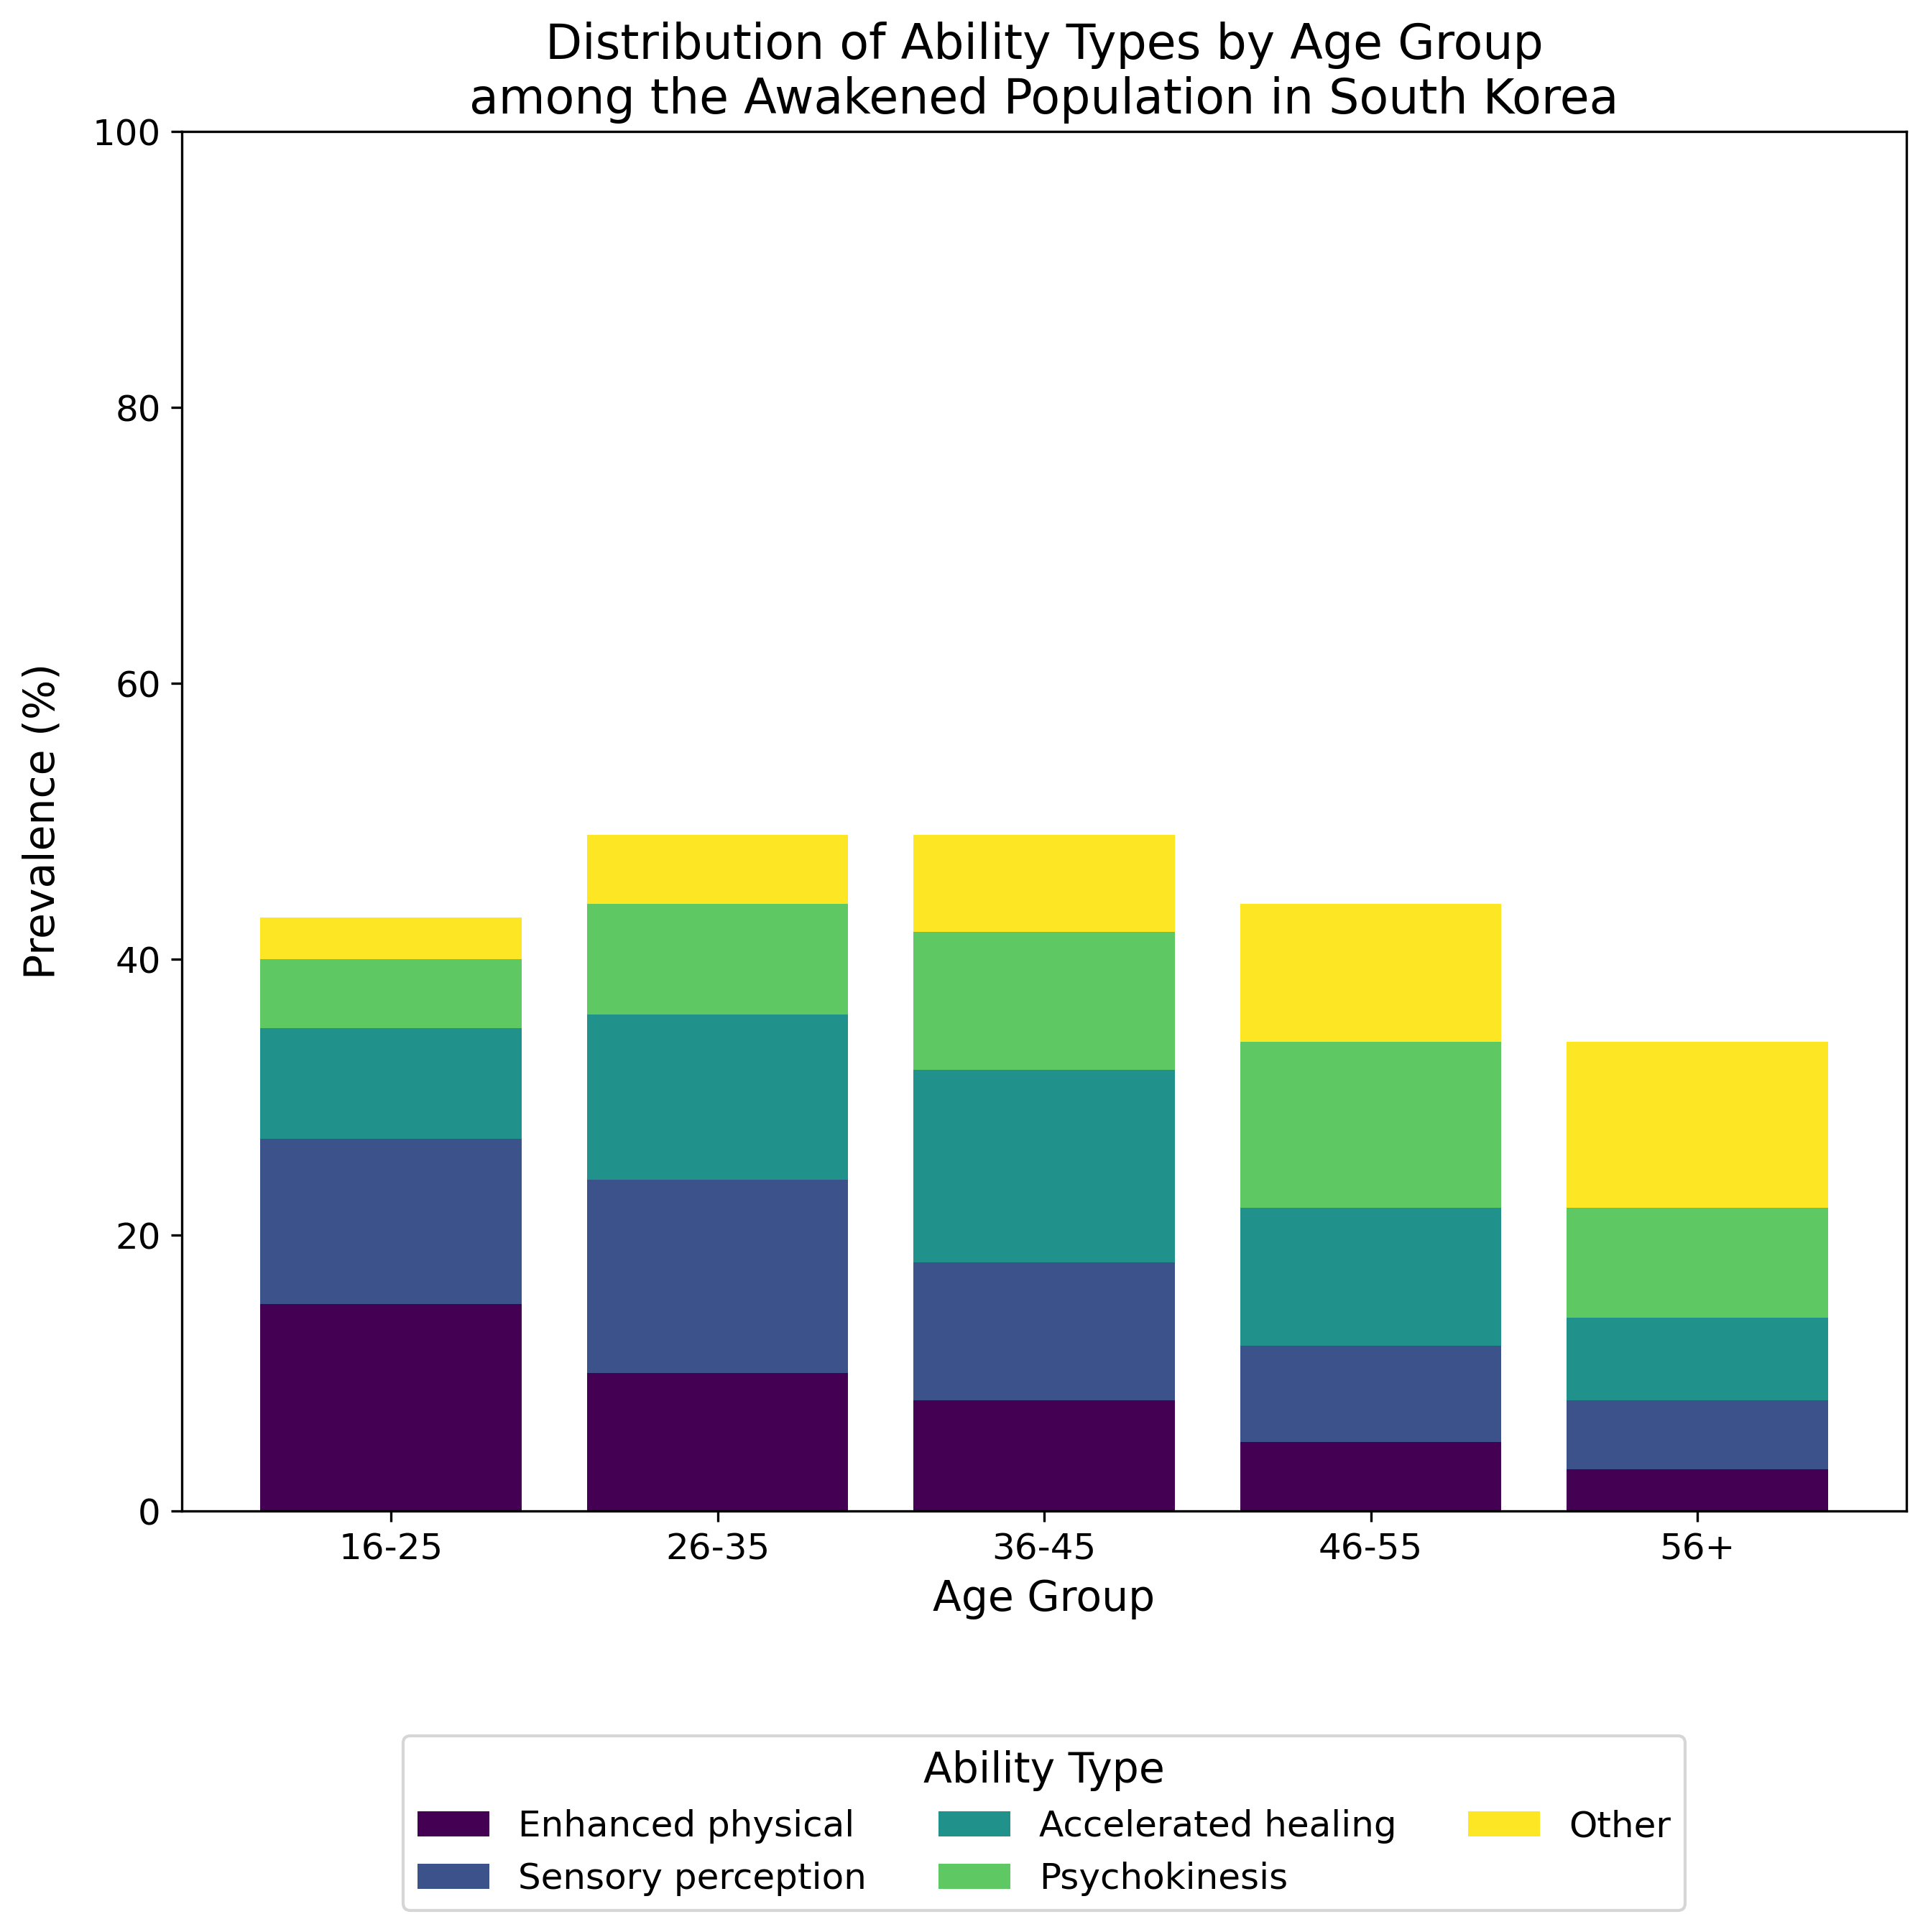
\includegraphics[width=0.8\textwidth]{ability_distribution.png}
    \caption{Distribution of ability types among the awakened population in South Korea.}
    \label{fig:ability_dist}
\end{figure}

Figure \ref{fig:ability_dist} presents the distribution of the most common ability types among the awakened population in South Korea. The prevalence of enhanced physical abilities and heightened sensory perception suggests that these may be foundational abilities that are more likely to manifest across a wider range of individuals. In contrast, the rarity of abilities such as reality manipulation and time control points to their exceptional nature and potential link to specific genetic or environmental factors.

% Table of ability types and their prevalence
\begin{table}[h]
\centering
\begin{tabular}{lc}
\hline
Ability Type & Prevalence (\%) \\
\hline
Enhanced physical strength & 32 \\
Heightened sensory perception & 28 \\
Accelerated healing & 24 \\
Psychokinesis & 17 \\
Elemental manipulation & 6 \\
Telepathy & 4 \\
Precognition & 2 \\
Reality manipulation & 1 \\
Time control & 1 \\
Interdimensional travel & 0.5 \\
Other & 15 \\
\hline
\end{tabular}
\caption{Prevalence of ability types among the awakened population in South Korea.}
\label{tab:ability_prev}
\end{table}

Table \ref{tab:ability_prev} provides a summary of the prevalence of the most common ability types among the awakened population. The "Other" category includes a diverse range of less common abilities, such as technopathy, animal communication, and astral projection. The wide variety of abilities reported by the participants highlights the complexity and diversity of the awakened population's supernatural capabilities.

\subsection{Social Integration Challenges}
The interview data revealed a range of challenges faced by the awakened population in South Korea in terms of social integration and acceptance. These challenges were grouped into three main themes: stigma and discrimination, pressure to conform, and lack of institutional support.

\subsubsection{Stigma and Discrimination}
Many interviewees reported experiencing stigma and discrimination due to their awakened status. They described instances of being treated as outsiders, facing fear and mistrust from non-awakened individuals, and being subjected to negative stereotypes and prejudices. Some participants recounted experiences of being denied employment, housing, or social services due to their abilities. As one interviewee stated:

\begin{quote}
    "People look at me like I'm a freak. They don't understand that I'm still the same person I was before I awakened. I've lost friends, and even some family members have distanced themselves from me." (Participant 7, male, age 28)
\end{quote}

These experiences of stigma and discrimination were particularly pronounced among individuals with more visible or unconventional abilities, such as those with physical transformations or abilities that challenge societal norms.

\subsubsection{Pressure to Conform}
Another common challenge reported by the interviewees was the pressure to conform to societal expectations and norms. Many participants felt that they were expected to suppress or hide their abilities to fit in and avoid drawing attention to themselves. They described the constant need to navigate social situations carefully and monitor their behavior to avoid making others uncomfortable or fearful. As one participant explained:

\begin{quote}
    "I feel like I have to constantly hold back and censor myself. I can't just be who I am because people might not accept me. It's exhausting always having to worry about how others will react to my abilities." (Participant 15, female, age 35)
\end{quote}

This pressure to conform was particularly challenging for individuals whose abilities were central to their identity and sense of self. Some interviewees expressed frustration at the lack of understanding and acceptance of their unique experiences and perspectives.

\subsubsection{Lack of Institutional Support}
Many interviewees also highlighted the lack of institutional support for the awakened population in South Korea. They described a dearth of resources, services, and policies tailored to their specific needs and challenges. Participants reported difficulties in accessing healthcare, mental health support, and legal assistance that takes into account their unique circumstances. As one interviewee noted:

\begin{quote}
    "There are no specialized clinics or therapists who understand what it's like to be awakened. I've had doctors dismiss my concerns or treat me like a curiosity. It's hard to find the support I need." (Participant 23, non-binary, age 42)
\end{quote}

Some interviewees also expressed frustration at the lack of legal protections against discrimination and the absence of policies that promote the inclusion and participation of the awakened in society. They called for greater recognition of their rights and needs at the institutional level.

\subsection{Coping Strategies and Resilience}
Despite the challenges faced by the awakened population, the interview data also revealed a range of coping strategies and sources of resilience. These included seeking support from within the awakened community, engaging in activism and advocacy, and finding meaning and purpose in their abilities.

Many interviewees described the importance of connecting with other awakened individuals and forming supportive networks. They spoke of the sense of belonging and understanding they found within the awakened community, which provided a space for them to share their experiences, learn from each other, and build solidarity. As one participant stated:

\begin{quote}
    "Being part of the awakened community has been a lifeline for me. It's the one place where I feel truly accepted and understood. We support each other and fight for our rights together." (Participant 11, female, age 29)
\end{quote}

Some interviewees also reported engaging in activism and advocacy as a way of coping with the challenges they faced. They described participating in community organizing, public education campaigns, and lobbying efforts to raise awareness of the needs and rights of the awakened population. These activities provided a sense of empowerment and purpose, as well as a means of effecting social change.

Finally, many participants spoke of finding meaning and purpose in their abilities, despite the challenges they posed. They described using their abilities to help others, contribute to society, and push the boundaries of what is possible. As one interviewee expressed:

\begin{quote}
    "My abilities have given me a unique perspective and a sense of responsibility. I know I have the power to make a difference, and that motivates me to keep going even when things get tough." (Participant 19, male, age 45)
\end{quote}

These coping strategies and sources of resilience highlight the strength and adaptability of the awakened population in the face of significant social and institutional barriers.

\section{Discussion}
The findings of this study provide valuable insights into the demographic characteristics, ability distribution, and social integration challenges of the awakened population in South Korea. The results highlight the diversity of this population segment, with a wide range of ages, genders, socioeconomic backgrounds, and ability types represented. The prevalence of certain abilities, such as enhanced physical strength and heightened sensory perception, suggests that these may be foundational abilities that are more likely to manifest across a broader spectrum of individuals.

However, the study also reveals significant challenges faced by the awakened population in terms of social integration and acceptance. The experiences of stigma, discrimination, and pressure to conform reported by the interviewees underscore the need for greater understanding, inclusion, and support for this unique population segment. The lack of institutional support and tailored resources identified by the participants points to the need for policy interventions and service provision that address the specific needs and challenges of the awakened.

At the same time, the coping strategies and sources of resilience described by the interviewees highlight the strength and adaptability of the awakened population. The importance of community support, activism, and finding meaning in one's abilities suggests potential avenues for fostering the well-being and empowerment of this population segment.

The findings of this study have implications for policymakers, service providers, and researchers working with the awakened population in South Korea. The results underscore the need for targeted interventions and support services that address the unique needs and challenges of this population segment, such as specialized healthcare, mental health support, and legal assistance. The development of policies and programs that promote the inclusion, participation, and rights of the awakened in society is also crucial.

Furthermore, the study highlights the importance of public education and awareness-raising efforts to combat stigma and discrimination against the awakened population. Initiatives that promote a more nuanced and understanding public discourse around the experiences and abilities of the awakened can help foster greater social acceptance and integration.

Finally, the findings of this study point to the need for further research on the awakened population in South Korea and beyond. Further investigations into the factors that shape the manifestation and distribution of abilities, the long-term impacts of awakening on individuals and society, and the effectiveness of different support and intervention strategies can help inform evidence-based policies and practices.

\section{Conclusion}
This study provides a comprehensive analysis of the awakened population in South Korea, shedding light on their demographic characteristics, ability distribution, and social integration challenges. The findings highlight the diversity and complexity of this unique population segment, as well as the significant barriers they face in terms of stigma, discrimination, and lack of institutional support.

However, the study also reveals the resilience and adaptability of the awakened population, as evidenced by their coping strategies and sources of strength. The importance of community support, activism, and finding meaning in one's abilities points to potential avenues for fostering the well-being and empowerment of this population segment.

The implications of this study are far-reaching, underscoring the need for targeted interventions, support services, and policies that address the unique needs and challenges of the awakened population. Public education and awareness-raising efforts are also crucial in combating stigma and promoting greater social acceptance and integration.

As the world continues to grapple with the profound impacts of the 2025 catastrophe and the emergence of the awakened population, studies such as this one provide valuable insights into the experiences, challenges, and resilience of this unique population segment. Further research and collaborative efforts across disciplines and sectors will be essential in developing evidence-based strategies to support the well-being and inclusion of the awakened population in South Korea and beyond.

\newpage

\bibliographystyle{apalike}
\bibliography{references}

\end{document}
